%LTeX: language=it
\subsection{UC 7 - Modifica di un oggetto} \label{sec:UC7}
    \begin{figure}[h]
        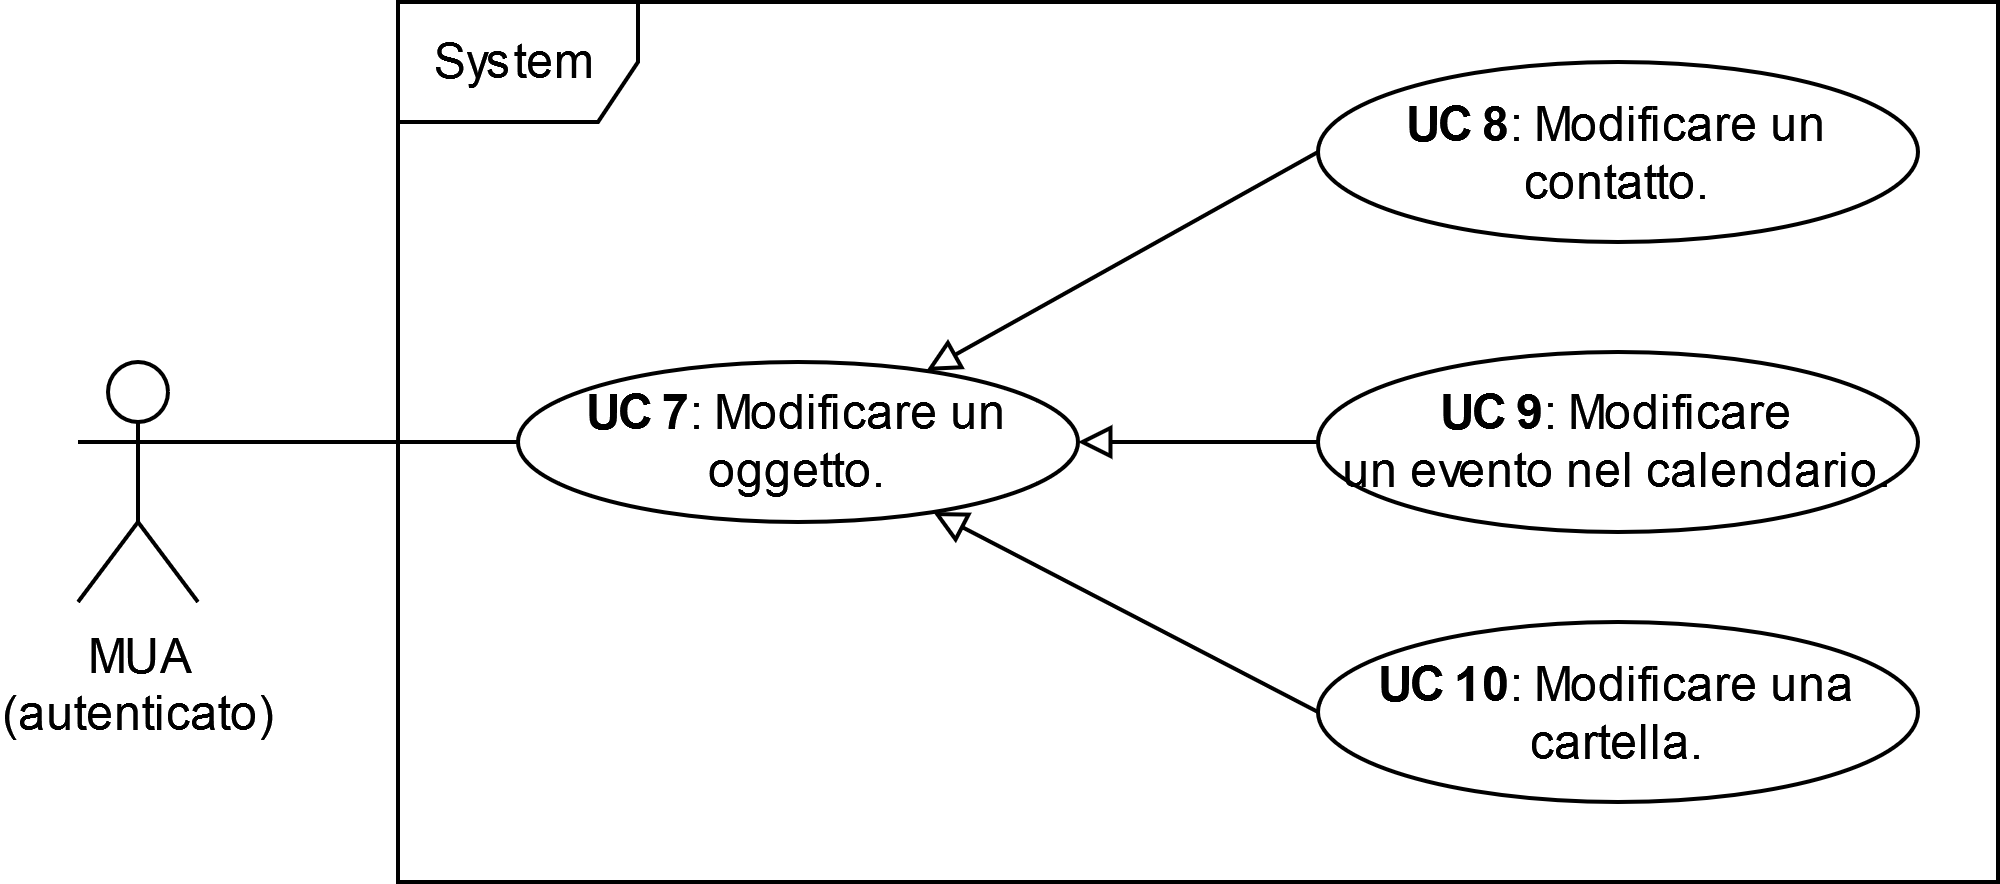
\includegraphics[width=0.85\textwidth]{sections/uc_imgs/UC07.png}
        \centering
        \caption{Diagramma UC 7.}
    \end{figure}
    \begin{itemize}
        \item \textbf{Attore principale}: MUA;
        \item \textbf{Descrizione}: il MUA deve poter modificare un oggetto nel sistema;
        \item \textbf{Precondizioni}: l’account che il MUA gestisce è registrato nel sistema, e ha un connessione aperta con il sistema ed è autenticato;
        \item \textbf{Postcondizioni}: il MUA modifica un oggetto, il suo nuovo stato viene salvato nel sistema;
        \item \textbf{Scenario principale}:
            \begin{enumerate}
                \item il MUA invia le informazioni per aggiornare l'oggetto nel sistema;
                \item il sistema salva il nuovo stato dell'oggetto;
            \end{enumerate}
        \item \textbf{Inclusioni}: nessuna;
        \item \textbf{Generalizzazioni}:
            \begin{itemize}
                \item il MUA modifica un contatto (\hyperref[sec:UC8]{UC 8});
                \item il MUA modifica un evento nel calendario (\hyperref[sec:UC9]{UC 9});
                \item il MUA modifica una cartella (\hyperref[sec:UC10]{UC 10});
            \end{itemize}
        \item \textbf{Estensioni}: nessuna.
    \end{itemize}